\section{Introduzione e descrizione dell'apparato}
Per condurre l'esperienza ci siamo serviti di una Breadboard dotata di due boccole e di una griglia di fori in cui inserire i refori. La griglia è caratterizzata dalla presenza di quattro colonne indicate con i simboli "+" e "-", ciascuna equipotenziale, e altre venti colonne equipotenziali riga per riga, indicate con delle lettere, come mostrato nella figura sottostante.

\begin{figure}[h!]
    \centering
    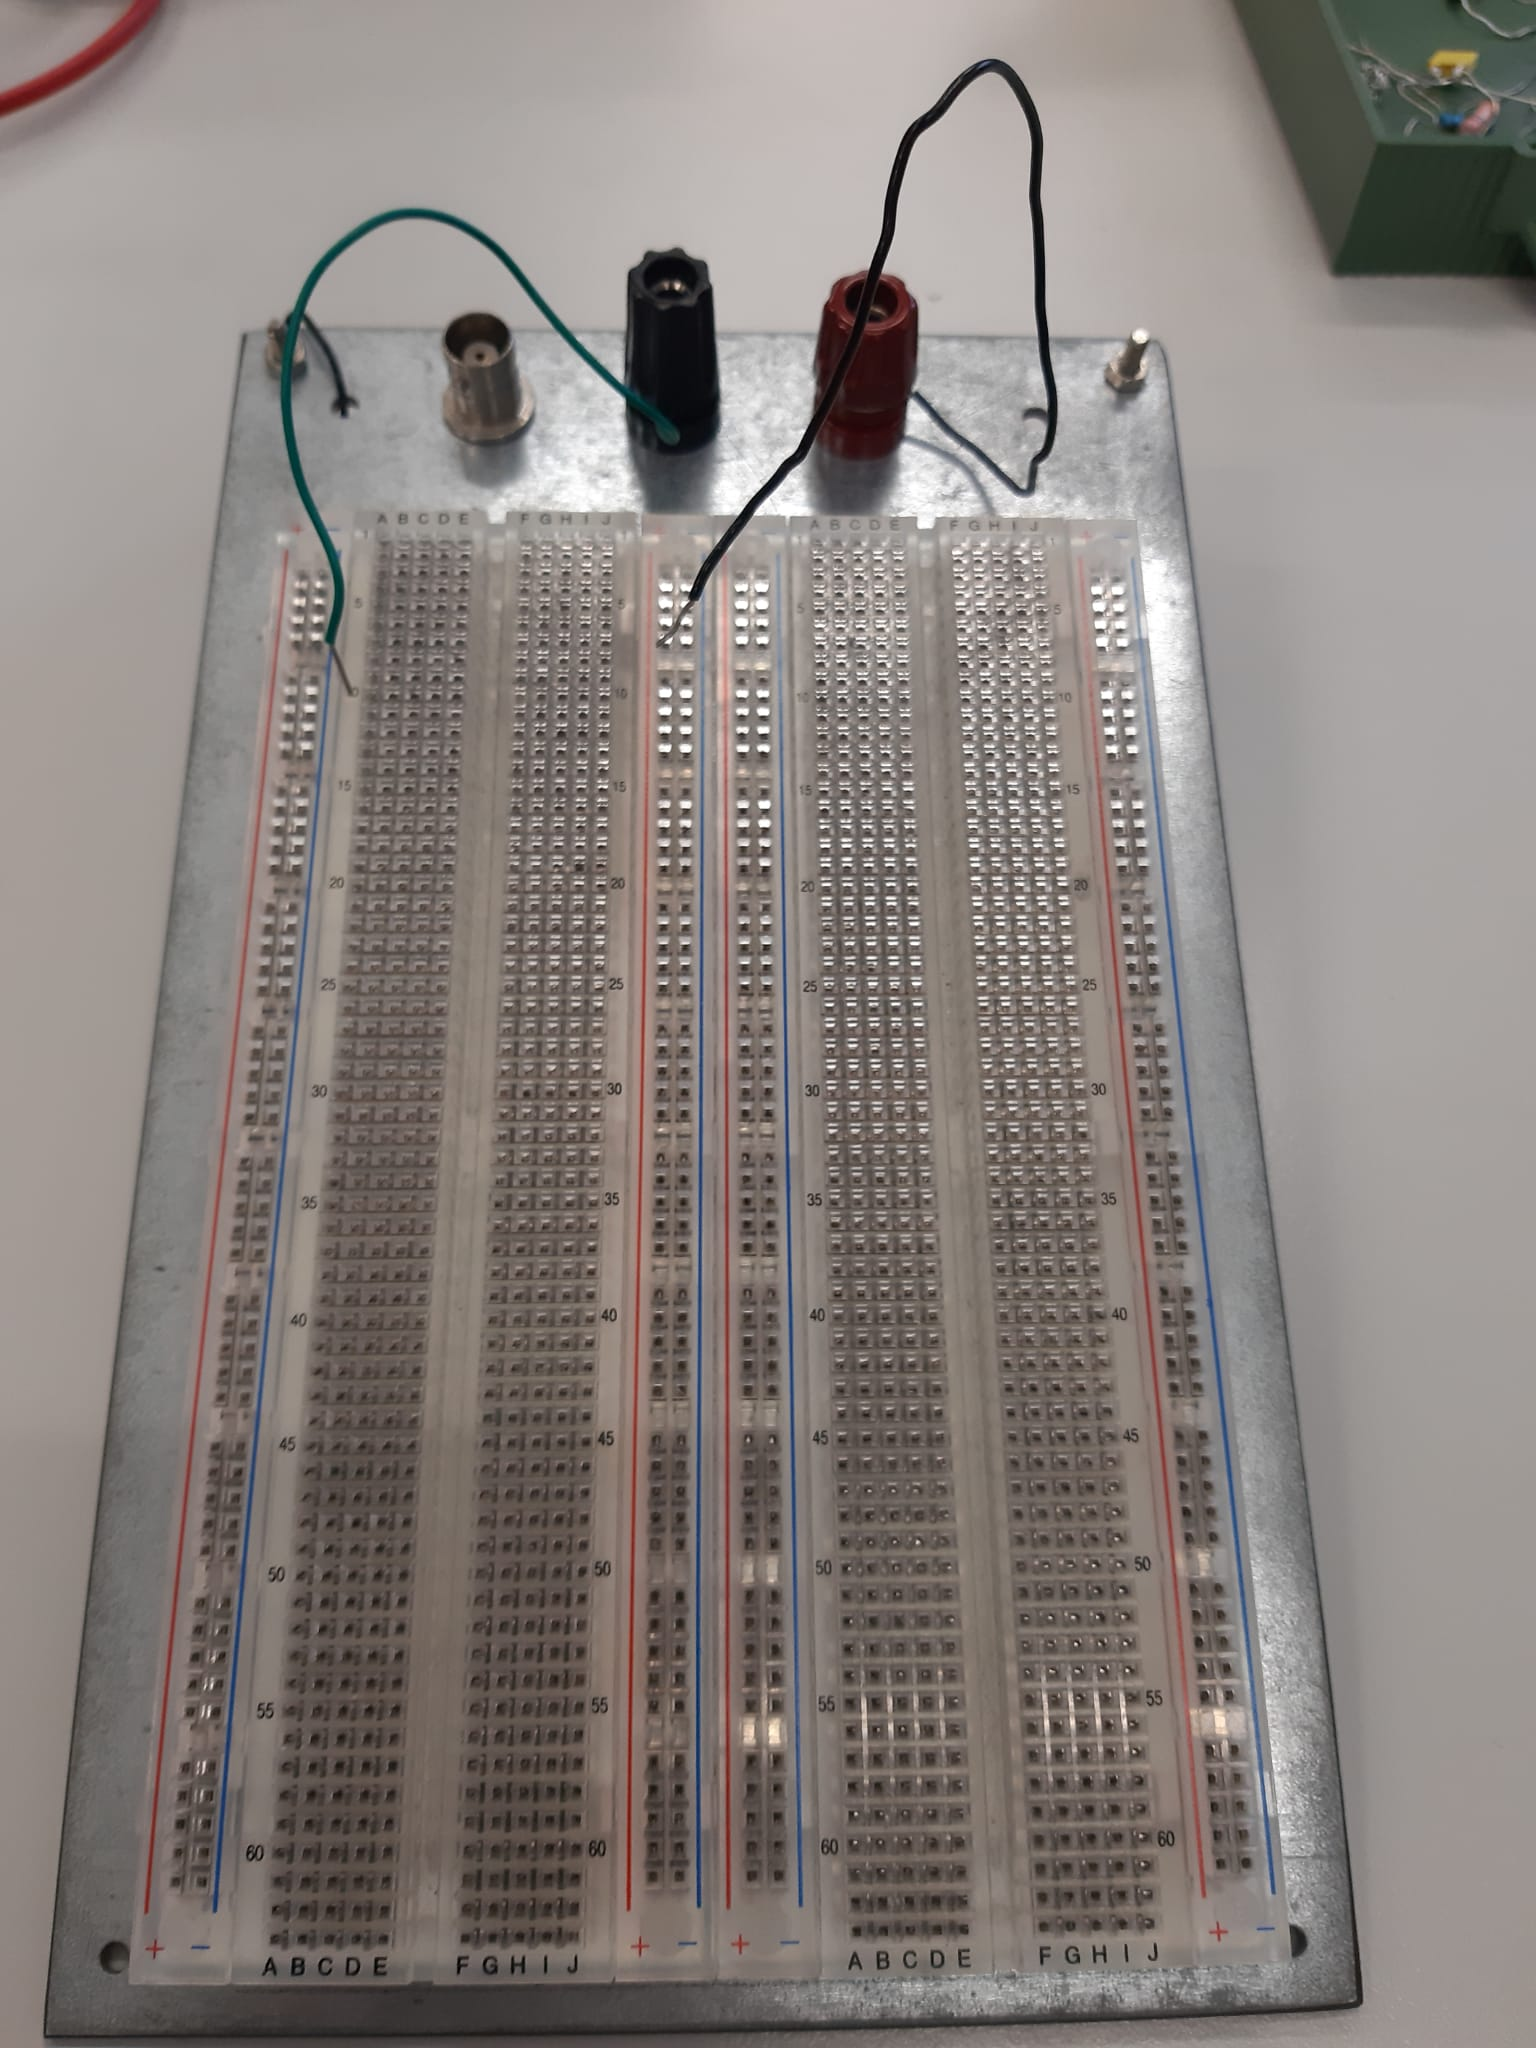
\includegraphics[scale=0.1]{Immagini/Circuitoooo.jpeg}
    \caption{}
\end{figure}

Lo strumento ci ha permesso di realizzare i circuiti su cui abbiamo condotto le diverse misure. Le componenti di circuito di cui ci siamo serviti sono state una resistenza, un condensatore e un induttore.
Abbiamo fatto uso di un generatore di segnali ad onde sinusoidali, delle quali era possibile modificare la frequenza e la tensione, che abbiamo tenuto fissa. Con un oscilloscopio siamo stati in grado di raccogliere le diverse misure ai capi delle componenti, dalle quali abbiamo ricavato parametri caratteristici.
Abbiamo articolato l'esperienza in 2 parti.
In primo luogo abbiamo studiato l'andamento delle funzioni di trasferimento per due circuiti: RC e RL.
Attraverso le impedenze, che sono rispettivamente $Z_{C} = \frac{1}{i \omega C}$ per la capacità e $Z_{L} = i \omega L$ per l'induttanza, abbiamo potuto risolvere i circuiti senza ricorrere alle equazioni differenziali.
Di conseguenza, la relazione $V_{g} = R_{TOT}I$ diventa $V_{g} = Z_{TOT}I$, dove con $V_{g}$ si intende la tensione del generatore. Per ogni componente valgono le seguenti relazioni:
$V_{C} = Z_{C}I$,   $V_{L} = Z_{L}I$,   $V_{R} = RI$.
Attraverso la prima si ricava $I = \frac{V_{g}}{Z_{TOT}}$, dalla quale è possibile ottenere la funzione di trasferimento H, una funzione complessa:

\begin{equation}
H=\frac{V_{i}}{V_{g}}=\frac{Z_{i}}{Z_{TOT}}
\end{equation}

Nello specifico, nel nostro caso si ottengono:
$$
H(\omega): V_{A} \rightarrow V_{A-B}
$$
\begin{equation}
|H(\omega)|=\left|\dfrac{V_{A-B}}{V_{A}}\right| 
\quad
arg[H(\omega)] = \Delta \phi'
\end{equation}
$$
H(\omega): V_{A} \rightarrow V_{B}
$$
\begin{equation}
|H(\omega)|=\left|\frac{V_{B}}{V_{A}}\right| \quad
arg[H(\omega)] = \Delta \phi'' \hspace{10}
\end{equation}


Anche per la seconda parte dell'esperimento abbiamo utilizzato le impedenze sopra descritte. L'impedenza totale ci ha permesso di descrivere la configurazione, servendoci di una relazione lineare che tenesse conto della resistenza e delle due impedenze relative al condensatore e all'induttore.


